\documentclass[10pt]{article}\usepackage[]{graphicx}\usepackage[]{xcolor}
% maxwidth is the original width if it is less than linewidth
% otherwise use linewidth (to make sure the graphics do not exceed the margin)
\makeatletter
\def\maxwidth{ %
  \ifdim\Gin@nat@width>\linewidth
    \linewidth
  \else
    \Gin@nat@width
  \fi
}
\makeatother

\definecolor{fgcolor}{rgb}{0.345, 0.345, 0.345}
\newcommand{\hlnum}[1]{\textcolor[rgb]{0.686,0.059,0.569}{#1}}%
\newcommand{\hlstr}[1]{\textcolor[rgb]{0.192,0.494,0.8}{#1}}%
\newcommand{\hlcom}[1]{\textcolor[rgb]{0.678,0.584,0.686}{\textit{#1}}}%
\newcommand{\hlopt}[1]{\textcolor[rgb]{0,0,0}{#1}}%
\newcommand{\hlstd}[1]{\textcolor[rgb]{0.345,0.345,0.345}{#1}}%
\newcommand{\hlkwa}[1]{\textcolor[rgb]{0.161,0.373,0.58}{\textbf{#1}}}%
\newcommand{\hlkwb}[1]{\textcolor[rgb]{0.69,0.353,0.396}{#1}}%
\newcommand{\hlkwc}[1]{\textcolor[rgb]{0.333,0.667,0.333}{#1}}%
\newcommand{\hlkwd}[1]{\textcolor[rgb]{0.737,0.353,0.396}{\textbf{#1}}}%
\let\hlipl\hlkwb

\usepackage{framed}
\makeatletter
\newenvironment{kframe}{%
 \def\at@end@of@kframe{}%
 \ifinner\ifhmode%
  \def\at@end@of@kframe{\end{minipage}}%
  \begin{minipage}{\columnwidth}%
 \fi\fi%
 \def\FrameCommand##1{\hskip\@totalleftmargin \hskip-\fboxsep
 \colorbox{shadecolor}{##1}\hskip-\fboxsep
     % There is no \\@totalrightmargin, so:
     \hskip-\linewidth \hskip-\@totalleftmargin \hskip\columnwidth}%
 \MakeFramed {\advance\hsize-\width
   \@totalleftmargin\z@ \linewidth\hsize
   \@setminipage}}%
 {\par\unskip\endMakeFramed%
 \at@end@of@kframe}
\makeatother

\definecolor{shadecolor}{rgb}{.97, .97, .97}
\definecolor{messagecolor}{rgb}{0, 0, 0}
\definecolor{warningcolor}{rgb}{1, 0, 1}
\definecolor{errorcolor}{rgb}{1, 0, 0}
\newenvironment{knitrout}{}{} % an empty environment to be redefined in TeX

\usepackage{alltt}
\usepackage[left=1in,right=1in,top=1in,bottom=1in]{geometry}
\usepackage{amsmath}
\usepackage{hyperref}
\usepackage{float}



\IfFileExists{upquote.sty}{\usepackage{upquote}}{}
\begin{document}

\title{STAT 405/605 Project}
\author{Sarvesh Fotedar, Ekrem Kizilkaya, Abbas Shaikh, Cody VanZandt, Andy Wang}
\maketitle
\tableofcontents

\newpage

\section{First Plots}

\subsection{Plot 1: Checkouts by Usage Class}
Figure \ref{fig:1} shows the number of physical and digital checkouts from the Seattle Public Library from 2018 to 2022. While the number of digital checkouts has shown consistent and steady growth within this time period, the number of physical checkouts per year has been more sporadic. Most notably, there was significant decrease of physical checkouts in 2020, most likely due to the onset of the COVID-19 pandemic, and the number of physical checkouts per year after 2020 has still not recovered to the levels seen in 2018 and 2019. Because of this downturn in physical checkouts, there were more digital than physical checkouts in years 2020 and 2021.
\begin{figure}[H]
\begin{center}
\begin{knitrout}
\definecolor{shadecolor}{rgb}{0.969, 0.969, 0.969}\color{fgcolor}
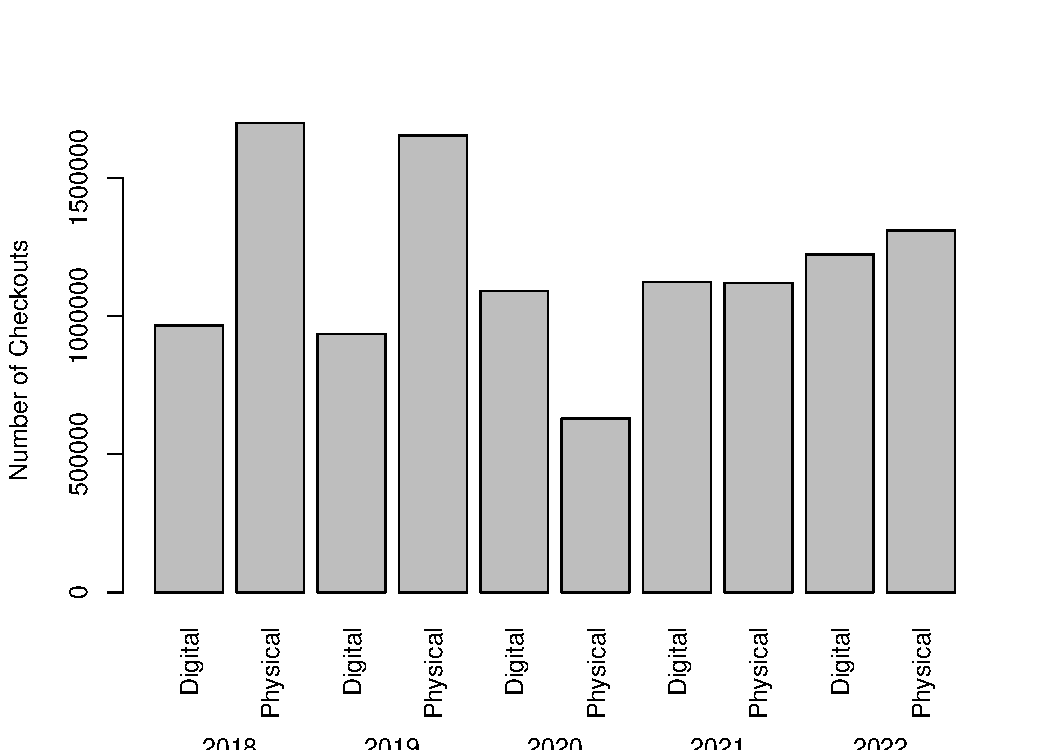
\includegraphics[width=\maxwidth]{figure/plot1-1} 
\end{knitrout}
  \end{center}
\caption{Number of Checkouts by Usage Class (Physical or Digital) per Year from 2018 to 2022.}\label{fig:1}
\end{figure}

\subsection{Plot 2: Most Popular Subjects}

Figure \ref{fig:2} shows the seven most popular book subjects of all books checked out between 2018 and 2022 in descending order of frequency. Books can have multiple subjects, such as both "Fiction" and "Literature." Fiction is the most popular topic with a little over 2.5 million occurrences, and Nonfiction had around 1.5 million. This is unsurprising since fiction and nonfiction are broad identifiers. In addition, in this plot, subjects are re-counted when their corresponding book is checked out again.

\begin{figure}[H]
\begin{center}
\begin{knitrout}
\definecolor{shadecolor}{rgb}{0.969, 0.969, 0.969}\color{fgcolor}
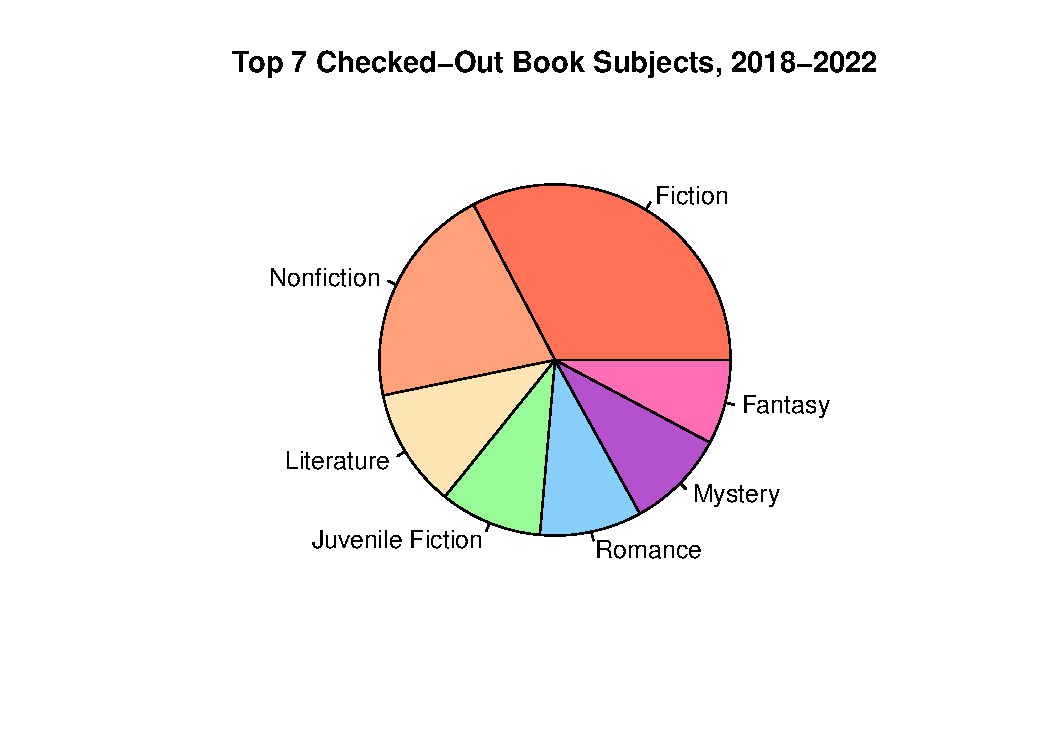
\includegraphics[width=\maxwidth]{figure/plot2-1} 
\end{knitrout}
\end{center}
\caption{Top 7 subjects of all books checked-out from 2018 to 2022.}\label{fig:2}
\end{figure}

\end{document}
